\begin{quote}
[Water waves] that are easily seen by everyone and which are usually
used as an example of waves in elementary courses [...] are the worst
possible example [...]; they have all the complications that waves can
have. \hfill (Richard Feynman, \textit{The Feynman Lectures on Physics})
\end{quote}

\section{Gravity waves}

Large waves, like those at the ocean, are driven by gravity. An
initial perturbation on the water surface, like an elevation, will
cause a rise in gravitational potenntial. As this energy is
transferred to kinetic energy, the water around it moves. Similarly to
a pendulum, an area below the mean surface will develop, which will be
filled with surrounding liquid. Thus, the perturbation travels away
from the initial disturbance.

The mathematical treatment of this problem is, in general, very
involved. This is mostly due to the presence of a free surface: the
water-air interface. Mathematically, its location is described by a
height function $\eta$:
\begin{equation}
  \label{eq:waves_elevation}
  z=\eta  \qquad  \eta=\eta(x,y,t) ,
\end{equation}
which is valid if no overhangs are present (this is known as a ``Monge
representation''). The fluid velocity is to be solved for a domain
between this surface at the ocean bottom, which is supposed to be flat
and at a height $z=-h$ (thus, $z=0$ is taken to be the surface when no
waves occur.)

We have the following boundary conditions for the velocity:
\begin{align}
  % p&=0 \\
  \label{eq:waves_bc}
  u_z(z=-h) &= 0 \\
  \label{eq:waves_bc2}
  u_z(z=0) &=  \frac{\partial \eta}{\partial t}
\end{align}


The first one is the usual condition at a solid wall, and the last one
is called the ``kinematic condition'', expressing the fact that if the
surface moves up or down, the fluid must do the same in order to be
``stuck to it''.

We will assume an incompressible, irrotational fluid. The fist
assumption is a very reasonable one, and the second one turns out to
be not so bad, since for small waves there is little vorticity
creation (it mainly occurs at the bottom and on breaking waves).  The
assumption of negligible viscosity is likewise not so bad in this
case.



Let us assume a wave train that only depends on the $x$ component
(i.e. waves are very long in the $y$ direction):

\begin{equation}
  \label{eq:wave_on_x}
  \eta = a \cos(kx -\omega t) .
\end{equation}
%
The amplitude $a$, is taken to be small (in the sense $a\ll \lambda$,
and $a\ll h$).

Given the assumptions above, the flow may be treated as a potential
flow, and moreover the only relevant coordinates will be $x$ and
$z$. However, the fields will be time-dependent in this problem,
e.g. $\phi=\phi(x,z,t)$.


The kinematic condition  implies
\[
\left. \frac{\partial \phi}{\partial z}\right|_{z=\eta} =
\frac{\partial \eta}{\partial t} .
\]
This is still a difficult expression, so we will approximate it by
\[
\left. \frac{\partial \phi}{\partial z}\right|_{z=0} =
\frac{\partial \eta}{\partial t} .
\]
(The difference between the two spactial derivatives may be quatified
by a Fourier expansion, in which the neglected terms are seen to be
higher order in $a$).

Let us consider the ansatz
\[
\phi = g(z) \sin(kx -\omega t ) .
\]
The kinematic condition then translates into $g'(0)=a\omega$.

The bottom condition clearly means
\[
\left. \frac{\partial \phi}{\partial z}\right|_{z= -h } = g'(-h)= 0 .
\]


All together, we are looking for a function with these boundary
conditions:
\begin{align}
  g'(0) &=  a \omega \\
  g'(-h) &= 0 .
\end{align}

However, the fact that Laplace equation must be satisfied places a
strong condition on the kind of function $g(z)$ may be:
\[
\nabla^2 \phi = 0 \qquad \implies \qquad
g''(z)  \sin(kx -\omega t ) - g(z)  k^2 \sin(kx -\omega t ) = 0 ,
\]
which meanse
\[
g''(z)  = k^2 g(z) .
\]
Therefore, $g(z)$ must be an exponential function, with the decay
constant being exactly equal to $k$, the wave number. In general, the
solution is a linear combination of two exponentials. Instead of that,
we may write another less conventional expression using hyperbolic
functions. This is equivalent, since these functions are themselves
linear combinaions of exponentials. Moreover, we choose to center them
at $x=-h$ :
\[
g(z)  = a_1 \cosh(k(z+h)) + a_2 \sinh(k(z+h)) .
\]
By inspection, we realize $a_2=0$, since the $\sinh(k(z+h))$ function
was the ``wrong'' behavior at $z=-h$: it has a slope, while the
boundary condition implies it should not.

The kinetic boundary condition implies
\[
a_1 = \frac{a \omega}{ k \sinh(hk)  } .
\]
This is indeed the only value for which $g'(0)= a \omega $. The
potential is then
\begin{equation}
  \label{eq:wave_potential}
  \phi = \frac{a \omega  \cosh(k(z+h)) }{ k \sinh( kh )  }  \sin(kx -\omega t ) .
\end{equation}

From it, the velocity components may be found. These will have a term
featuring $\sin(kx -\omega t )$, a common expression for a traveling
wave. However, the theory is still incomplete since $\omega$ and $k$
are not unrelated in a physical wave, but coupled by the phase
velocity $c=\omega / k$. Remember how in sound waves this velocity was
related to fluid compressibility (to be precise, the square root of
the variation of pressure with density). In this case, such
relationship is as yet missing. Also notice that gravity has played no
role whatsoever, despite claims at the beginning of this chapter about
this factor being the driving force behind this process.

In order to find the missing link, let us remember our previous
expression for the Bernoulli principle, Eq.~\ref{eq:Bern_unsteady},
which can be written as
\[
\frac{\partial \bfu}{\partial t} +
\nabla \cdot \left[
  \frac12 u^2 + \frac{p}{\rho} + \varphi
  \right] =  \frac{p}{\rho}\nabla \cdot \bfu .
\]

In our case the fluid is incompressible, so the right hand side
vanishes. Also, in potential flow we may write the whole equation
compactly:
\[
\nabla \cdot \left[
  \frac{\partial \phi}{\partial t} +
  \frac12 u^2 + \frac{p}{\rho} + \varphi
  \right] =  0 .
\]

This means the whole term on which the divergence operator acts
must be constant in space, but not in time in general:
\[
  \frac{\partial \phi}{\partial t} +
  \frac12 u^2 + \frac{p}{\rho} + \varphi =  f(t) .
\]
This is the less-known unsteady Bernoulli principle.

In this particular case, since boundary conditions do not change in
time (in fact, they do, but we are taking the surface to be close to
$z=0$), any function $f(t)$ may be incorporated into the potential
by making the following trick:
\[
\phi' = \phi + \int_{t_0}^t f(t') dt' ,
\]
hence we may just take $f(t)=0$ in this particular problem.

If we examine the ``head'' term, $ \partial \phi / \partial t +
\frac12 u^2 + \frac{p}{\rho} + \varphi$ at the surface, we notice that
the pressure should be constant (equal to atmospheric pressure, as in
hydrostatics). The $u^2$ may be neglected within our
assumptions. Last, but not least, gravity finally appears in the
potential, $\varphi = g \eta $. This leaves us with
\[
\left.\frac{\partial \phi}{\partial t}\right|_{z=0} + g \eta = 0 ,
\]
often called the ``dynamic condition''. 

With our previous result, this means:
\[
\phi =  - \frac{a \omega^2  \cosh(k(z+h)) }{ k \sinh(hk)  }  \cos(kx -\omega t ) +
g a \cos(kx -\omega t ) =0 .
\]

The result is the following dispersion relation:
\[
\omega^2= g k \tanh(k h)
\]
This is a surprising result, despite being obviously dimensionally
correct, whith the two lengths in the problem, $\lambda=2\pi/k$ and
$h$ providing the relevant lenght scales.



As a result, the phase velocity is then
\[
  c= \frac{\omega}{k} = \sqrt{ \frac{g}{k}  \tanh(k h) } ,
\]
while the group velocity, after some algebra is found to be
\[
  c_\mathrm{gr} := \frac{d\omega}{dk} =
  \frac{c}{2}
  \left(
    1 + kh \frac{1- \tanh^{2}(kh)}{\tanh(k h)}
  \right)
\]

\begin{figure}
  \centering
  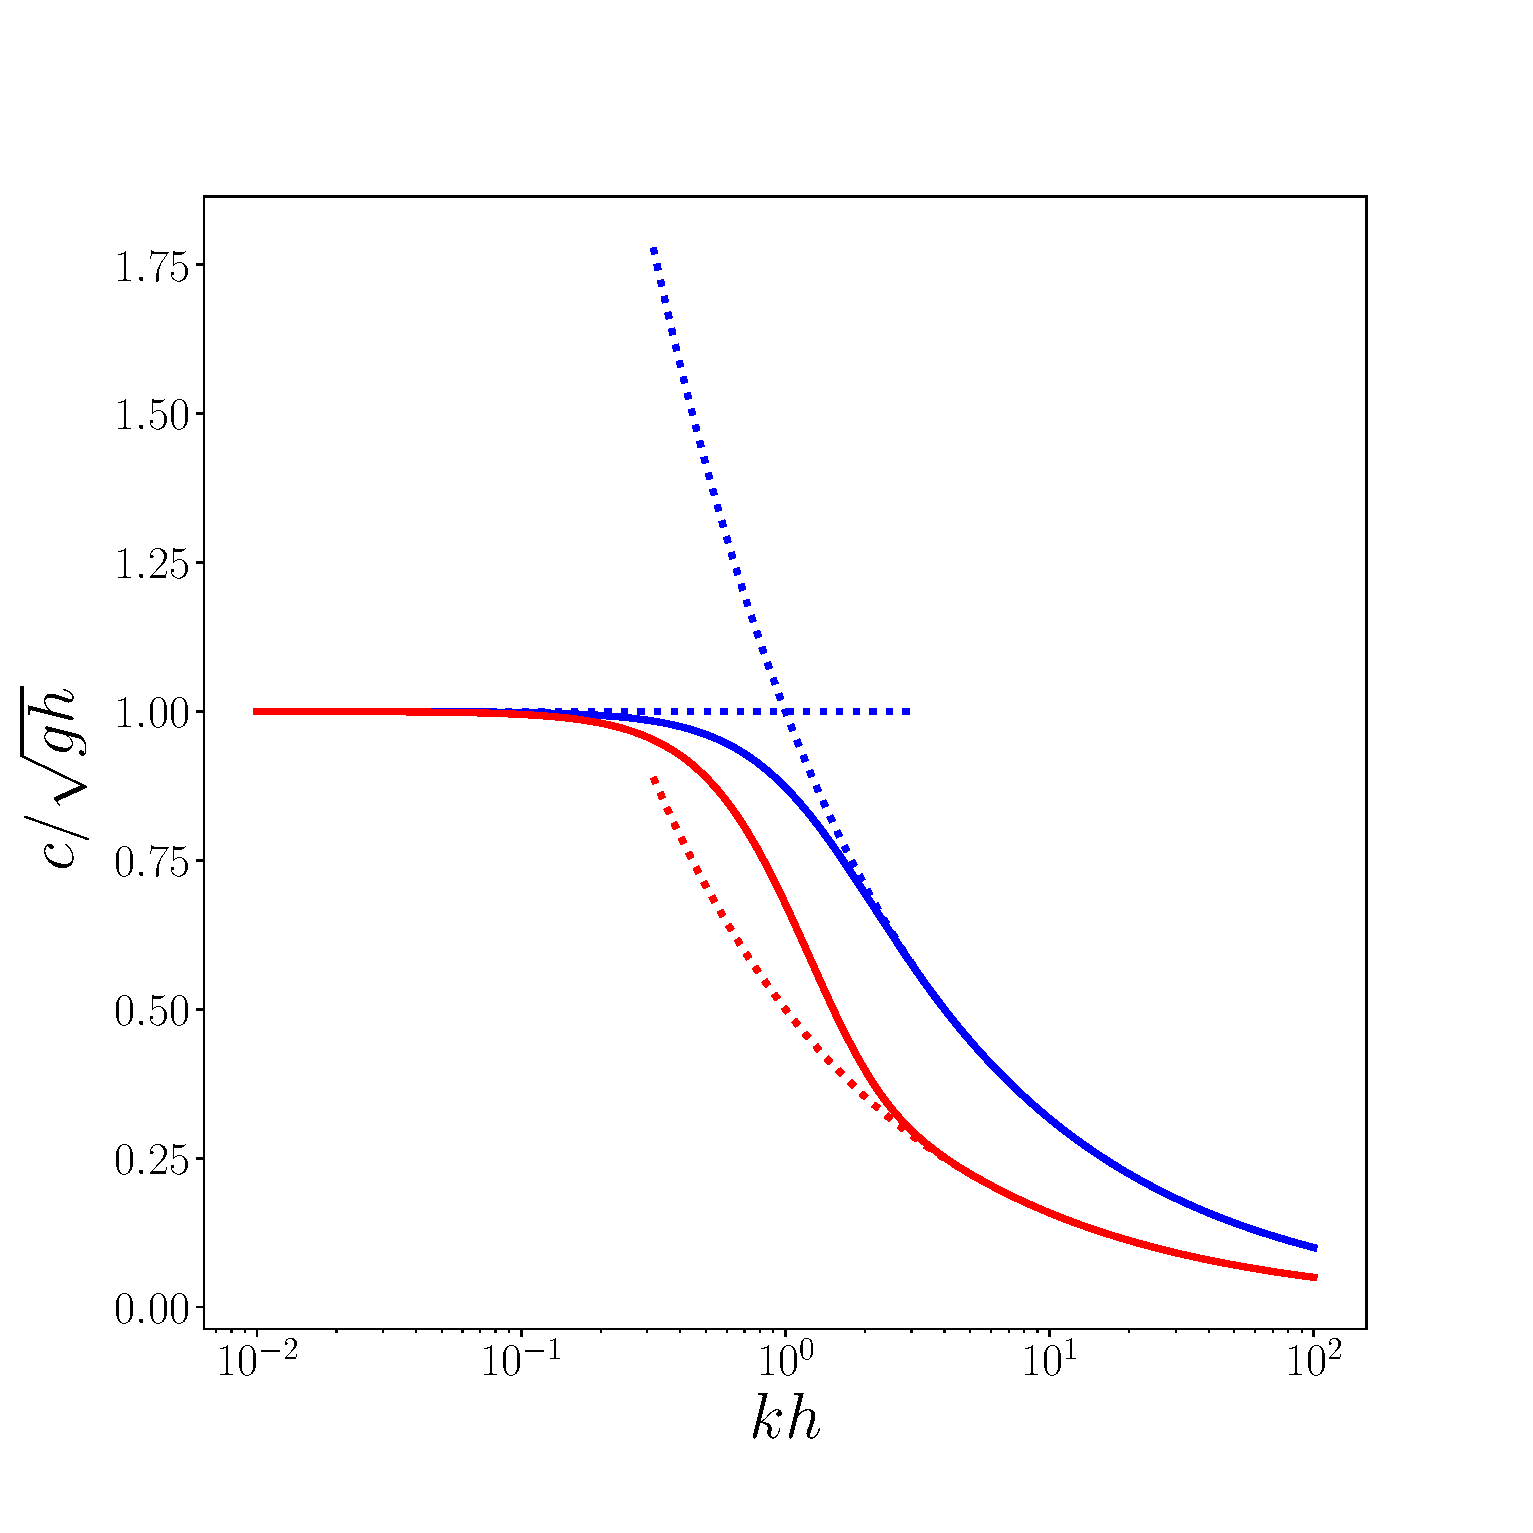
\includegraphics[width=0.4\linewidth]{figures/gravity_waves_disp}
  \caption{Dispersion relationship for gravity waves as a function of
    reduced wave-vector $kh$. \label{fig:gravity_waves_disp}}
\end{figure}

These two velocities are shown in \ref{fig:gravity_waves_disp}}. We
may distinguish two limits, which we discuss separately.

\subsection{Shallow water}
If the bottom is small, compared to the wavelength $\lambda$, then
$kh = 2\pi h / \lambda $ is a small number, and we may approximate
$\tanh(kh)\approx kh$. Then,
\[
\omega^2= g h  k^2 \qquad \implies \qquad \omega= k \sqrt{g h} .
\]

In this limit, the phase velocity is independent of velocity, which
means the process is non-dispersive:
\[
c =  \frac{\omega}{k} = \sqrt{ g h }  .
\]
The group velocity is of course equal to the phase velocity:
\[
c_\mathrm{g} := \frac{d\omega}{dk} = \sqrt{ g h } = c.
\]

The relevant length in this limit is the depth $h$, which provides the
correct dimensions to get a velocity.






Notice ``shallow'' is defined in relation to the wavelength. A seismic
wave may be excited at the deep sea by a geological process that may
involve tenths or hundreds of kilometers, much larger than the usual
sea depth, which is some few kilometers (its mean value is about
$\SI{3.8}{\kilo\meter}$.) The sea is then ``shallow'', and the speed
at which the perturbation travels will be about
\[
c \approx \sqrt{\SI{9.8}{\meter\per\second\squared} \times
  (\SI{4e3}{\meter}) } \approx \SI{200}{\meter\per\second}
  \approx \SI{700}{\kilo\meter\per\hour} 
\]
This is an astonishing speed, which is nevertheless in agreement with
measurements of these dramatic events.

\subsection{Deep water}

If the bottom is deep, compared to the wavelength $\lambda$, then $kh
= 2\pi h / \lambda $ is a large number, and its hyperbolic tangent is
very nearly $1$. In this limit,
\begin{equation}
  \label{eq:water_disp_deep}
  \omega^2 \approx g  k \qquad \implies \qquad \omega= \sqrt{g k} .
\end{equation}

These waves are highly dispersive, since their phase velocity depends
on the wavelength:
\[
c =  \frac{\omega}{k} = \sqrt{ g /k  } =  \sqrt{ g \lambda / (2\pi)  }  .
\]

The group velocity is now different from the phase velocity. In fact,
it is one half that value:
\[
2 \log\omega = \log k + \log g \qquad \implies \qquad
\frac{2}{\omega} \frac{d\omega}{dk} = \frac1{k} \qquad  \implies \qquad
c_\mathrm{g} = \frac{c}{2}
\]

In deep waters, the only two length scales we may think of are the
wave amplitude $a$ and their wavength $\lambda$. As we expect the
amplitude to play no role (as long as it is small, $a\ll\lambda$), we
are left with the wavelength to provide the length scale.

Notice that waves high high wavelenghts travel faster. This explains
the groundsell phenomenon, by which waves generated by a far away
storm may arrive quickly at some shore. These waves may precede the
storm by a long time, if the storm does arrive at all. The velocity
grows larger and larger with the wavelength, but as we have seen in
the previous section, as the wavelength becomes comparable to the
depth there will be a crossover to some finite velocity.

